\begin{frame}
  \frametitle{Hybrid $S_N$-Diffusion Method: 3-D Neutronics Eigenvalue Simulations}
  \begin{columns}
    \column{5.5cm}
  \textbf{3-D Full-Core MSRE Model}
  \begin{figure}[p]
    \centering
    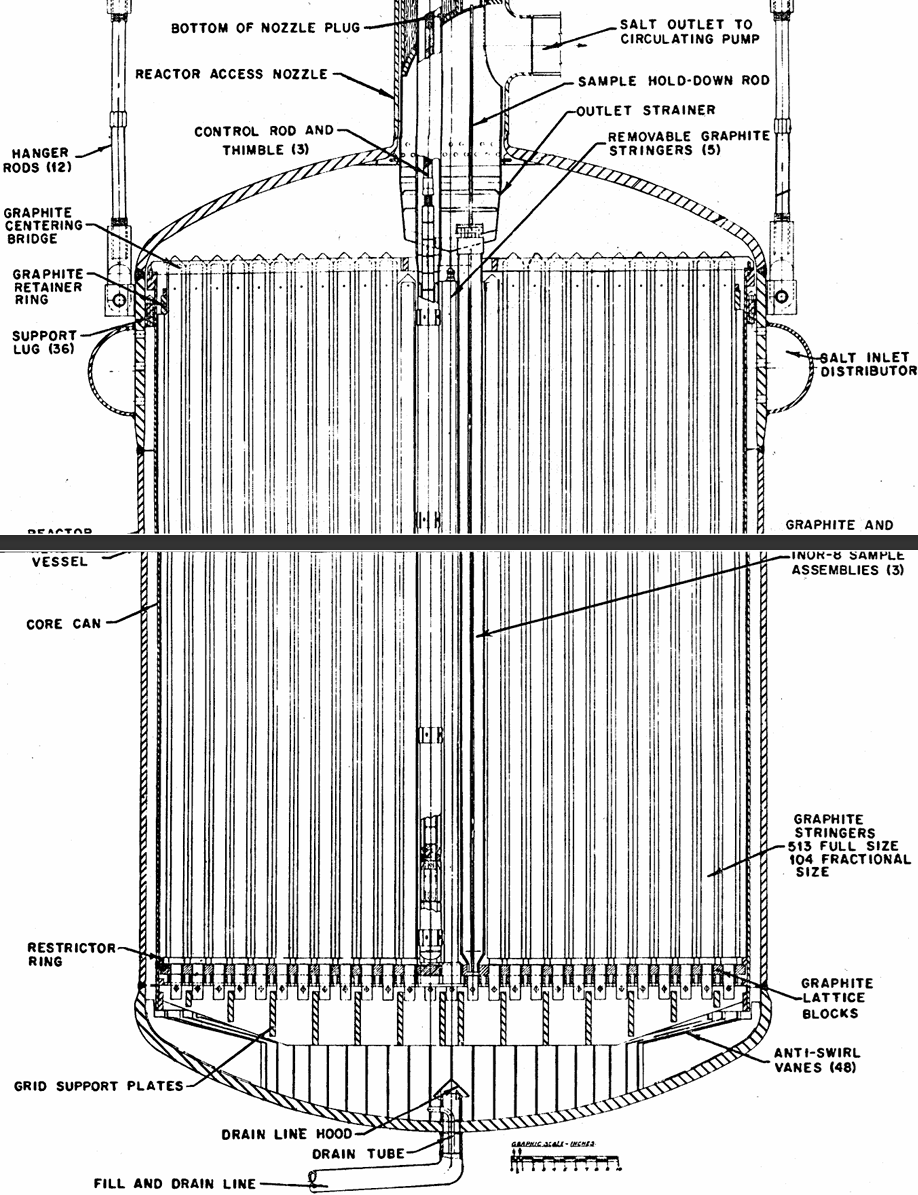
\includegraphics[width=0.85\columnwidth]{msre-picture}
    \caption{Vertical cross section of the actual \gls{MSRE} vessel.}
    \label{fig:msre-picture}
  \end{figure}
    \column{6cm}
  \begin{figure}[p]
    \centering
    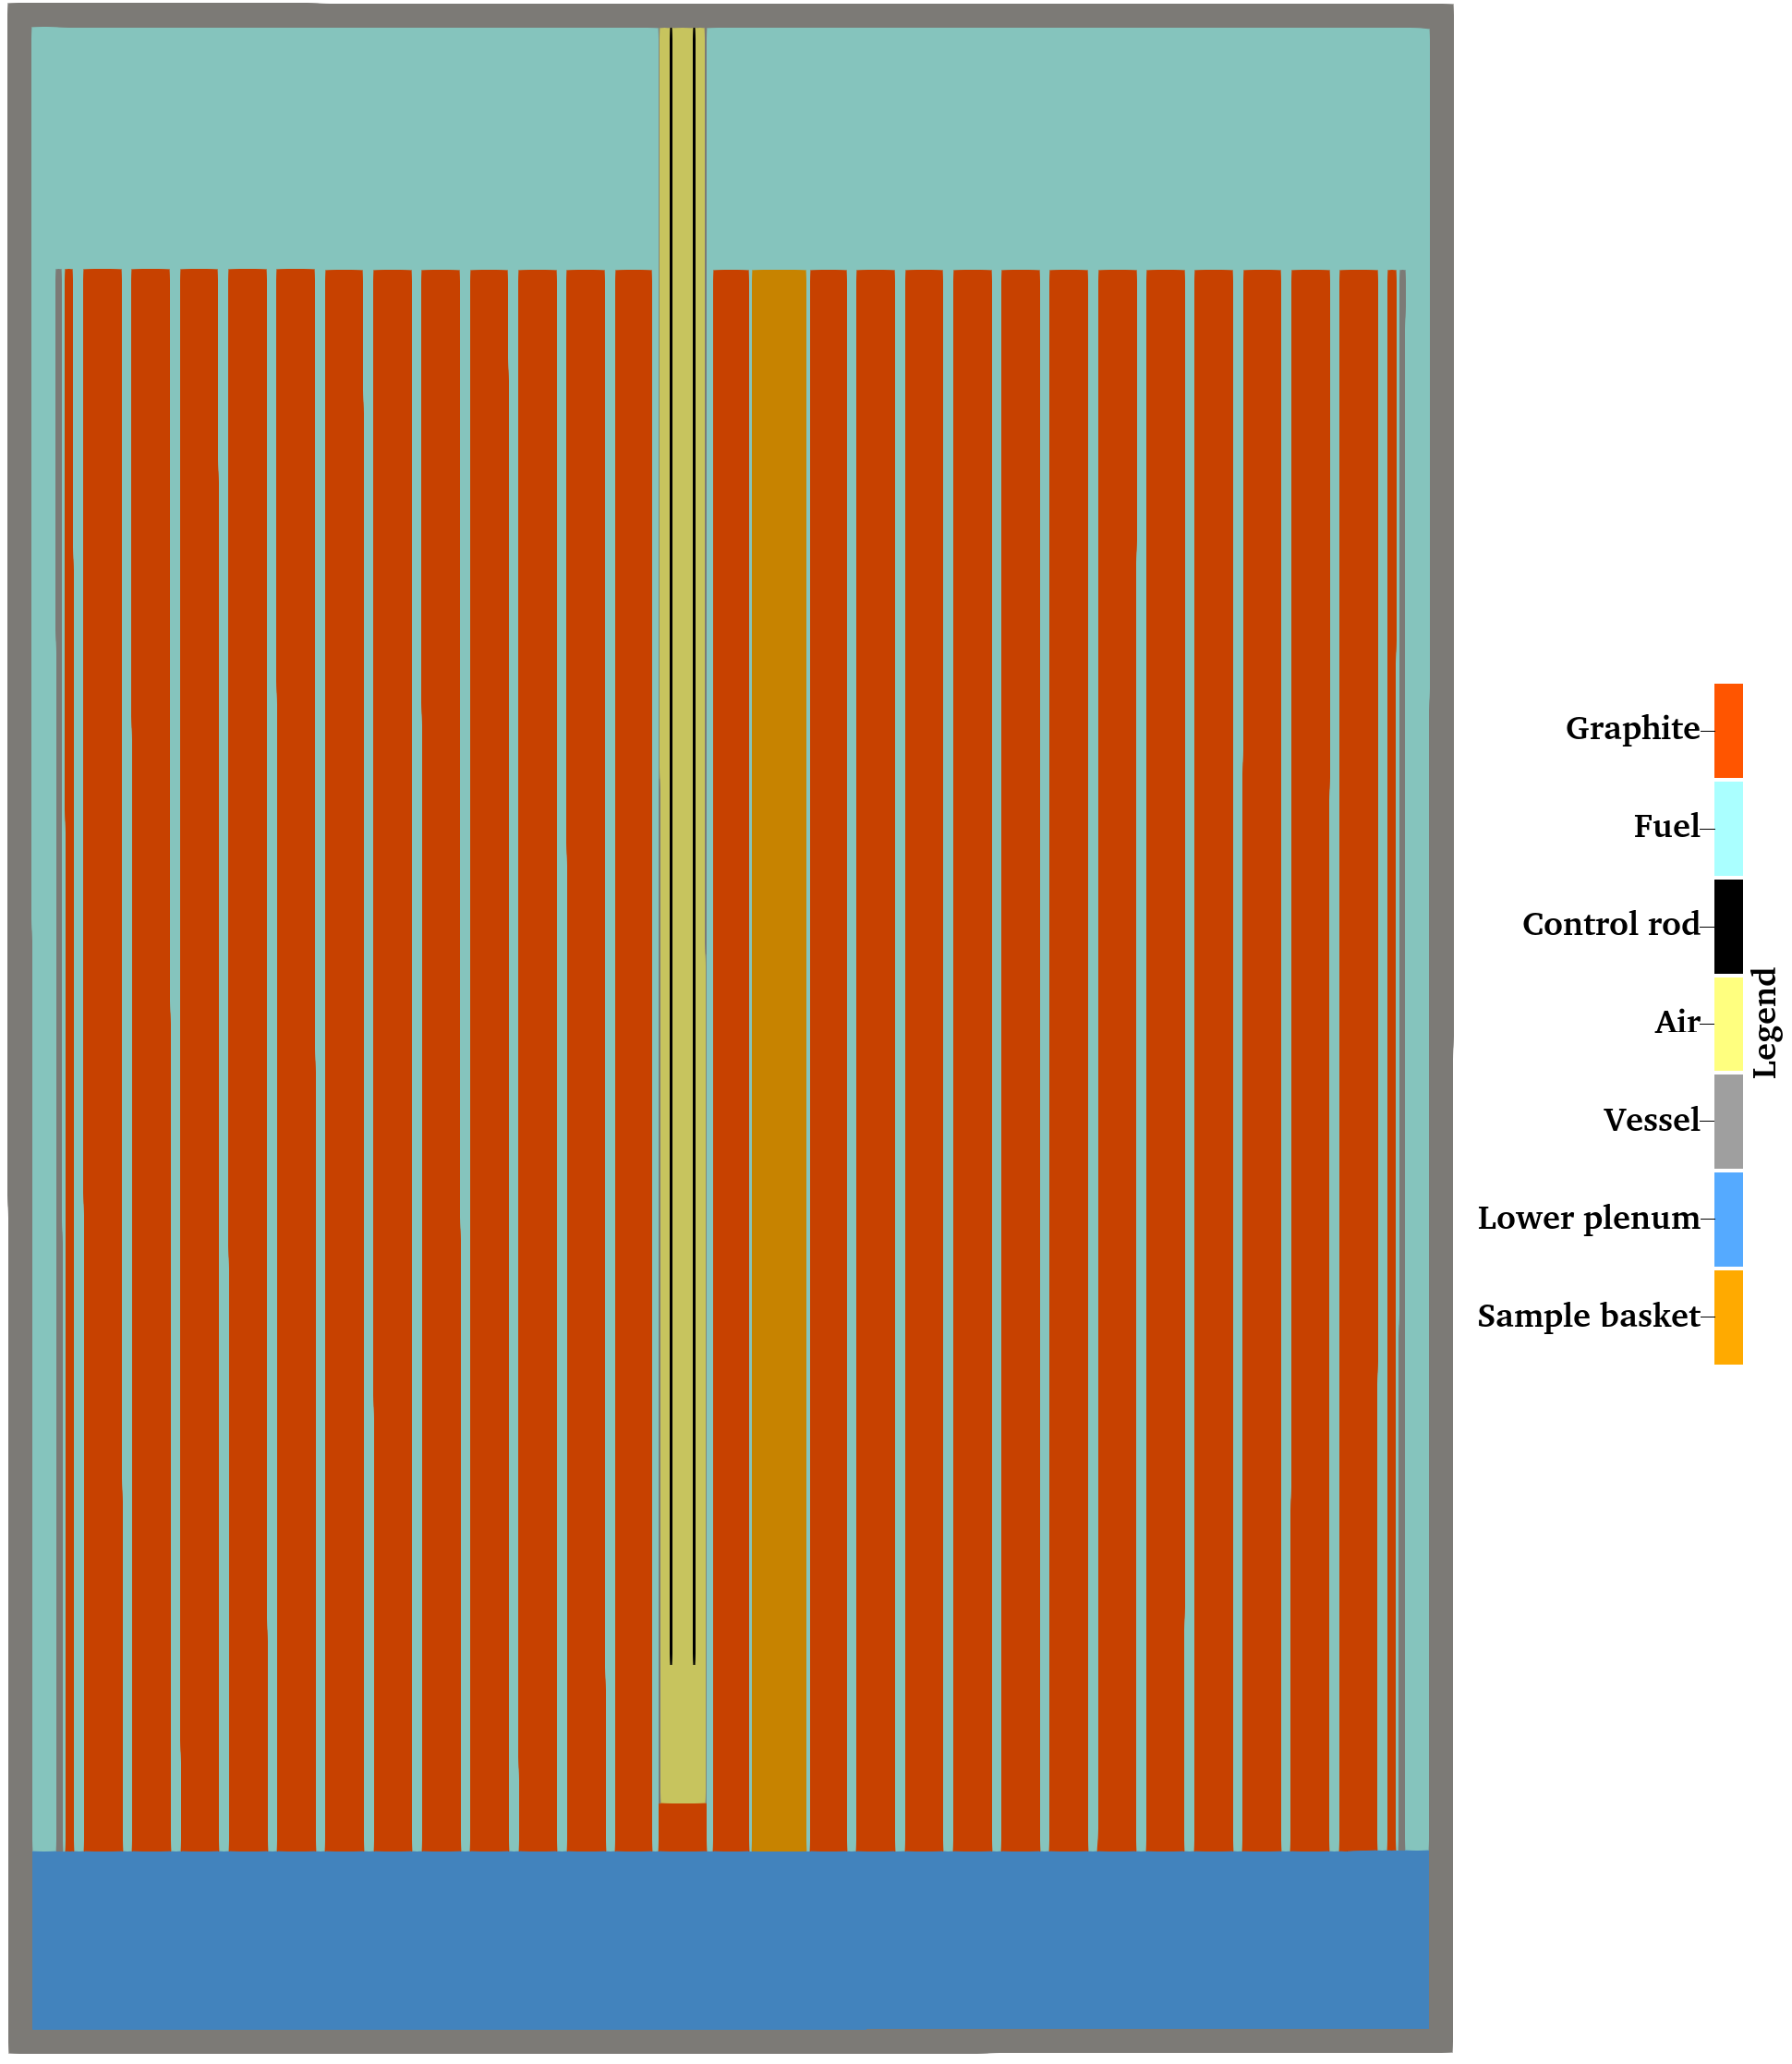
\includegraphics[width=.95\columnwidth]{msre-geom-vert}
    \caption{Vertical cross section of the 3-D numerical \gls{MSRE} model offset by 5.08 cm to show
    the control rod thimble and homogenized sample basket.}
    \label{fig:msre-geom-vert}
  \end{figure}
\end{columns}
\end{frame}

\begin{frame}
  \frametitle{Hybrid $S_N$-Diffusion Method: 3-D Neutronics Eigenvalue Simulations}
  \textbf{3-D Full-Core MSRE Model Details}
  \begin{itemize}
    \item Hybrid $S_6$-diffusion method
    \item $^{235}$U concentration at initial criticality
    \item Uniform temperature at 911 K
    \item Stabilization factor of $c=250$
    \item Void constant of $\varsigma=0.5$
    \item Uncorrected diffusion coefficient values capped at $D_g = 2.5$
  \end{itemize}
  \vspace{.2cm}

  These parameters are required for numerical stability in the air-filled control rod
  thimble region.
  \vspace{.2cm}

  All hybrid method results are compared with MSRE experimental data, the MSRE numerical benchmark
  report data (Serpent 2 model) \cite{fratoni_molten_2020}, and the OpenMC model in this work.
\end{frame}

\begin{frame}
  \frametitle{Hybrid $S_N$-Diffusion Method: 3-D Neutronics Eigenvalue Simulations}
  \textbf{MSRE at Initial Criticality}
  \begin{table}[htb]
    \centering
    \caption{$k_\text{eff}$ values from \gls{MSRE} experimental data, the \gls{MSRE} numerical
    benchmark \cite{fratoni_molten_2020}, and the OpenMC and Moltres models in this work.}
    \begin{tabular}{l S[table-format=1.5(2)]}
      \toprule
       & {$k_\text{eff}$} \\
       \midrule
      \gls{MSRE} experimental data & 1.00000(420) \\
      Serpent 2 (Numerical benchmark) & 1.02132(3) \\
      OpenMC (This work) & 1.01308(20) \\
      Hybrid (This work) & 1.01955 \\
      Diffusion (This work) & 1.01885 \\
      \bottomrule
    \end{tabular}
    \label{table:initial-crit}
  \end{table}

  \begin{itemize}
    \item The Serpent 2 benchmark model reports a $k_\text{eff}$ of 1.01093(3) after considering some
      of the geometrical modifications used in the OpenMC model.
    \item The hybrid and neutron diffusion models agree with the OpenMC model within 700 pcm.
  \end{itemize}
\end{frame}

\begin{frame}
  \frametitle{Hybrid $S_N$-Diffusion Method: 3-D Neutronics Eigenvalue Simulations}
  \textbf{MSRE Rod Worth Measurements}
  \begin{figure}[t]
    \centering
    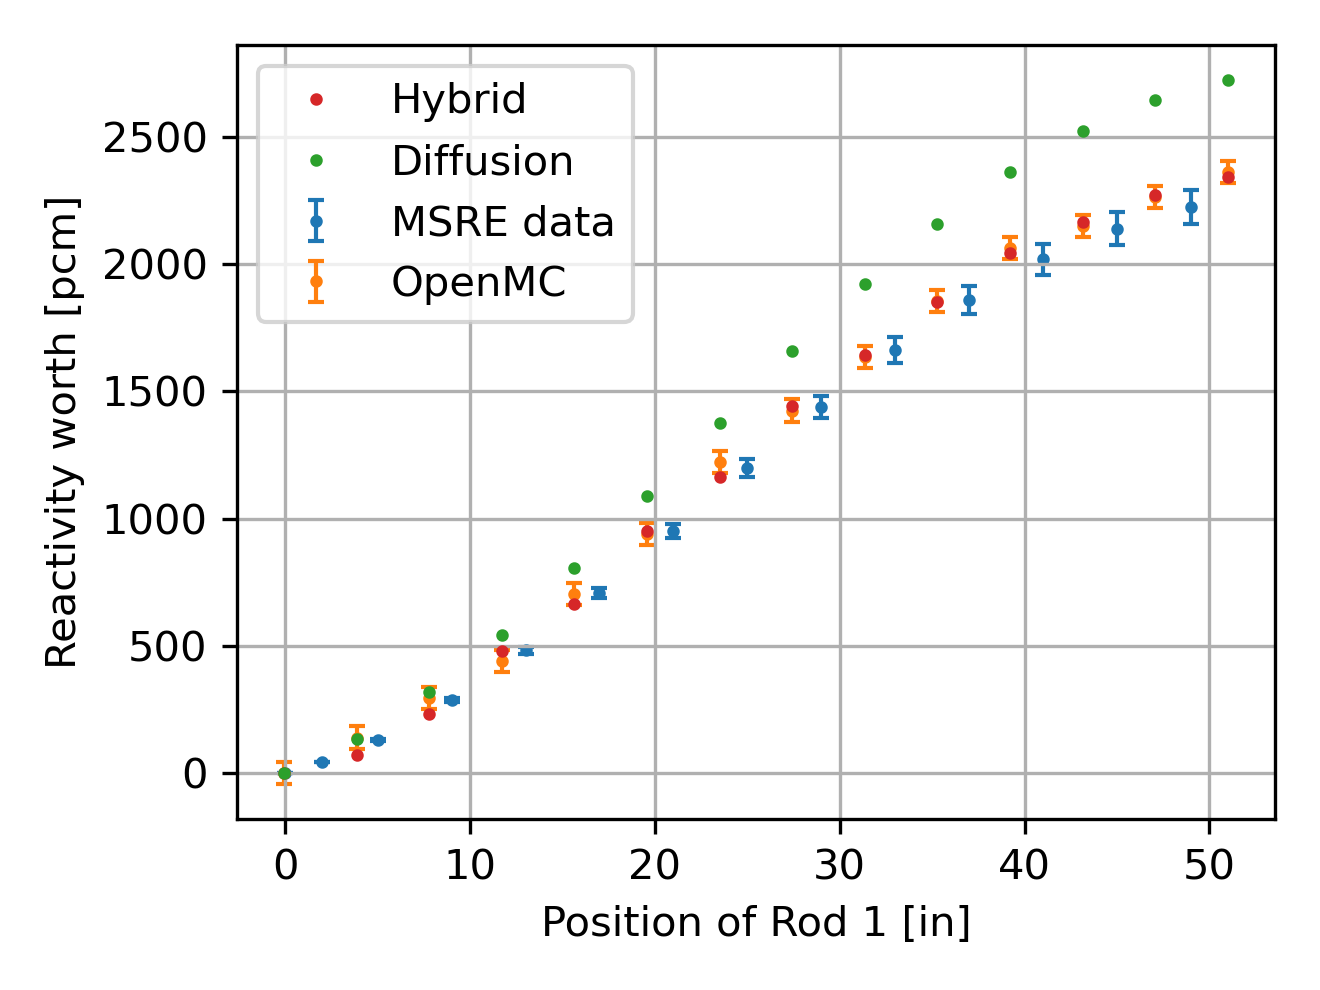
\includegraphics[width=0.8\columnwidth]{rod-worth-curve}
    \caption{Reactivity inserted by Rod 1 at various rod positions relative to the full insertion.}
    \label{fig:rod-worth}
  \end{figure}
\end{frame}

\begin{frame}
  \frametitle{Hybrid $S_N$-Diffusion Method: 3-D Neutronics Eigenvalue Simulations}
  \textbf{MSRE Rod Worth Measurements}
  \begin{table}[t]
    \centering
    \caption{Total rod worth of Rod 1 when fully inserted.}
    \begin{tabular}{l S[table-format=4(2)] S}
      \toprule
       & {$\rho_\text{worth}$ [pcm]} & {Percentage discrepancy [\%]}\\
       \cmidrule(rl){2-2} \cmidrule(l){3-3}
      \gls{MSRE} experimental data & 2250(67) & {-}\\
      OpenMC (This work) & 2364(44) & 5.1 \\
      Hybrid (This work) & 2345 & 4.2 \\
      Diffusion (This work) & 2725 & 21.1 \\
      \bottomrule
    \end{tabular}
    \label{table:rod-worth}
  \end{table}
  \vspace{.2cm}

  Slight overprediction by OpenMC and the hybrid method due to approximating the control rod
  as an annular cylinder instead of beaded rod elements.
  \begin{figure}[t]
    \begin{subfigure}[b]{0.22\columnwidth}
      \centering
      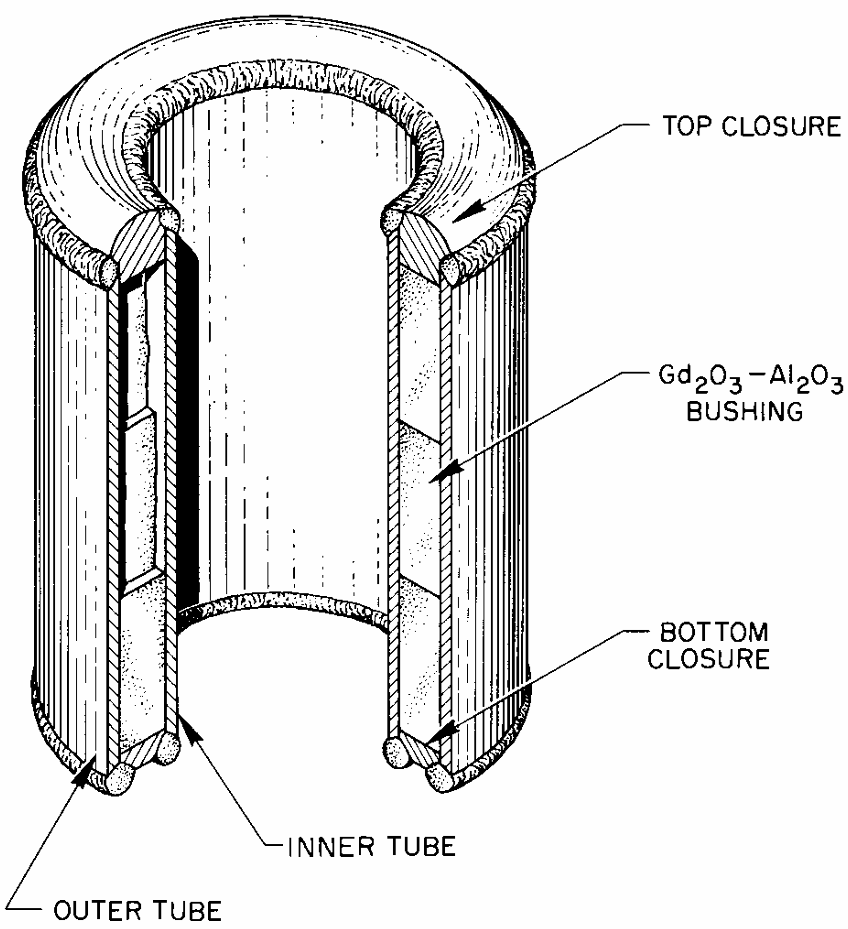
\includegraphics[width=\columnwidth]{rod-bead-2}
    \end{subfigure}
    \begin{subfigure}[b]{0.44\columnwidth}
      \centering
      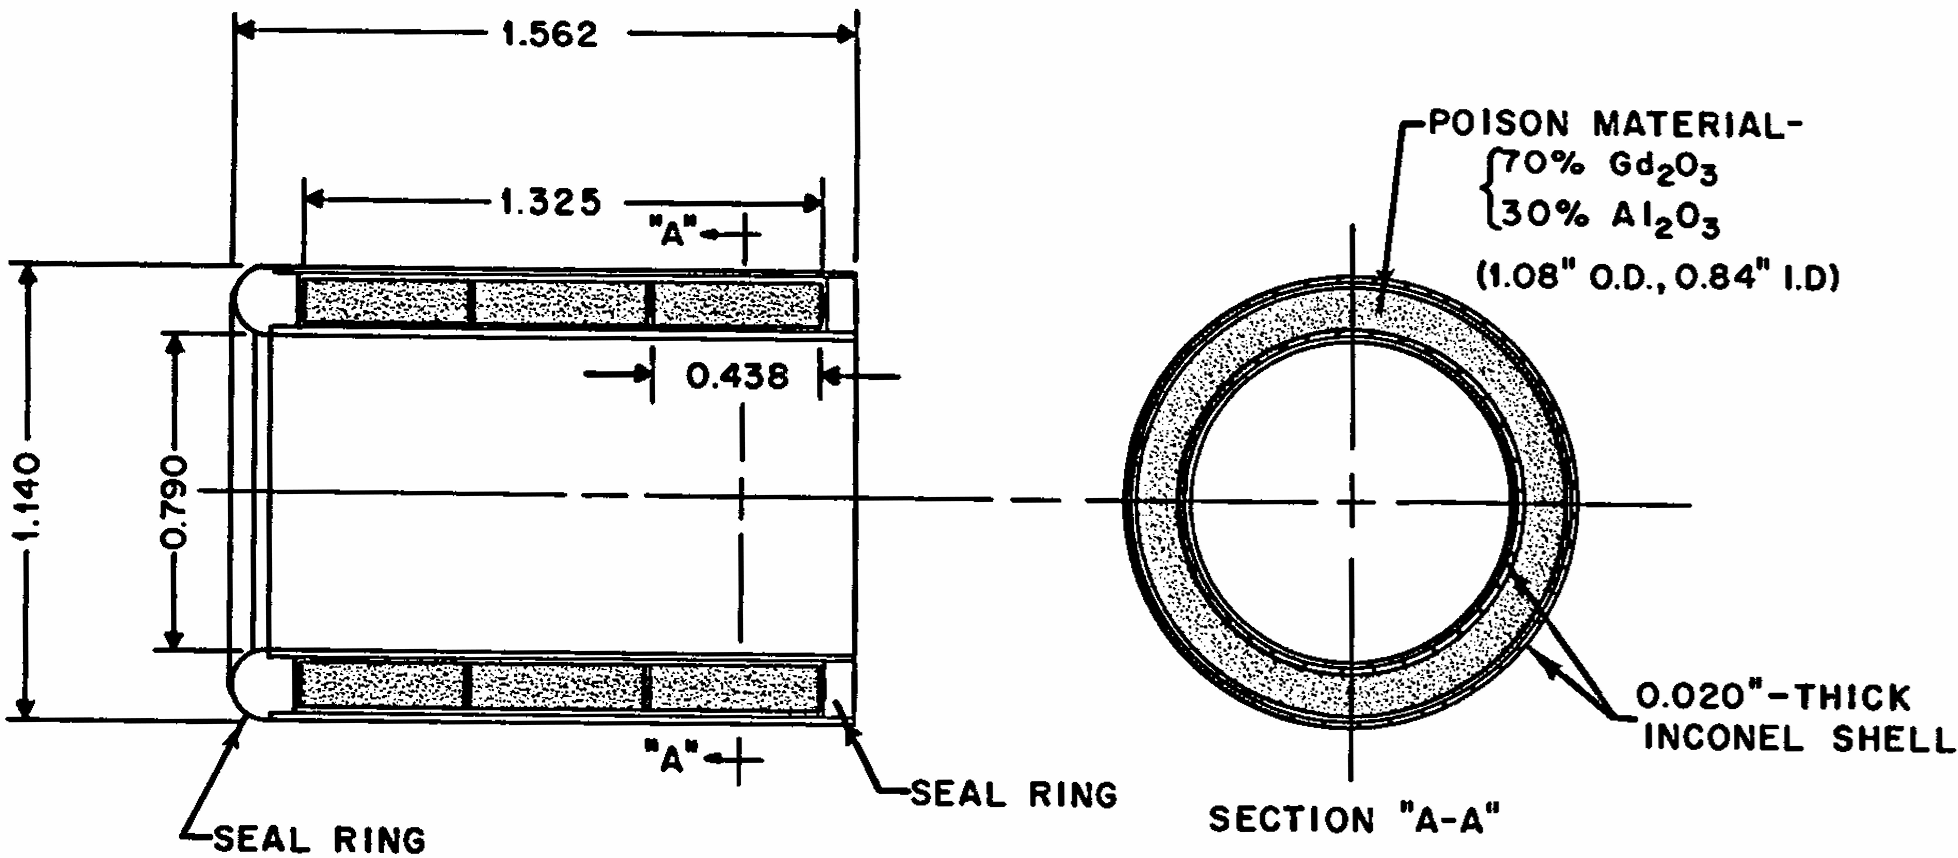
\includegraphics[width=\columnwidth]{rod-bead}
    \end{subfigure}
    \caption{Cutaway view and dimensions of a control rod poison element. Retrieved from
    \cite{tolson_msre_1967} and \cite{robertson_msre_1965}.}
    \label{fig:rod-bead}
  \end{figure}
\end{frame}

\begin{frame}
  \frametitle{Hybrid $S_N$-Diffusion Method: 3-D Neutronics Eigenvalue Simulations}
  \textbf{Computational Performance}
  \begin{itemize}
    \item All simulations ran on the Polaris supercomputer system at Argonne National Laboratory.
    \item Each 3-D full-core simulation consisted of 750M and 1.69B degrees of freedom for the
      neutron diffusion and $S_N$ subsolvers, respectively.
    \item 3-D full-core simulations required at least 40 compute nodes with 512 GB RAM each due to
      strict memory requirements (significant improvements in memory use is possible) and took 2.2
      h to complete.
    \item The hybrid method took about four times longer than the neutron diffusion method.
    \item 30 \% of compute time spent on data transfers between the neutron diffusion and $S_N$
      subsolvers (Reduced to 18 \% in subsequent simulations after optimizations)
  \end{itemize}
\end{frame}

\begin{frame}
  \frametitle{Hybrid $S_N$-Diffusion Method: 3-D Neutronics Eigenvalue Simulations}
  \textbf{Strong Scaling Test}
  \vspace{.2cm}

  Performed a strong scaling test on the 3-D quarter-core MSRE model on 10, 20, 40, and 80 compute
  nodes. The $S_N$ and diffusion subsolvers scale well throughout the test.
  The $S_N$-diffusion data transfer processes scale poorly beyond 40 nodes.
  \begin{figure}[t]
    \centering
    \begin{subfigure}[b]{0.32\columnwidth}
      \centering
      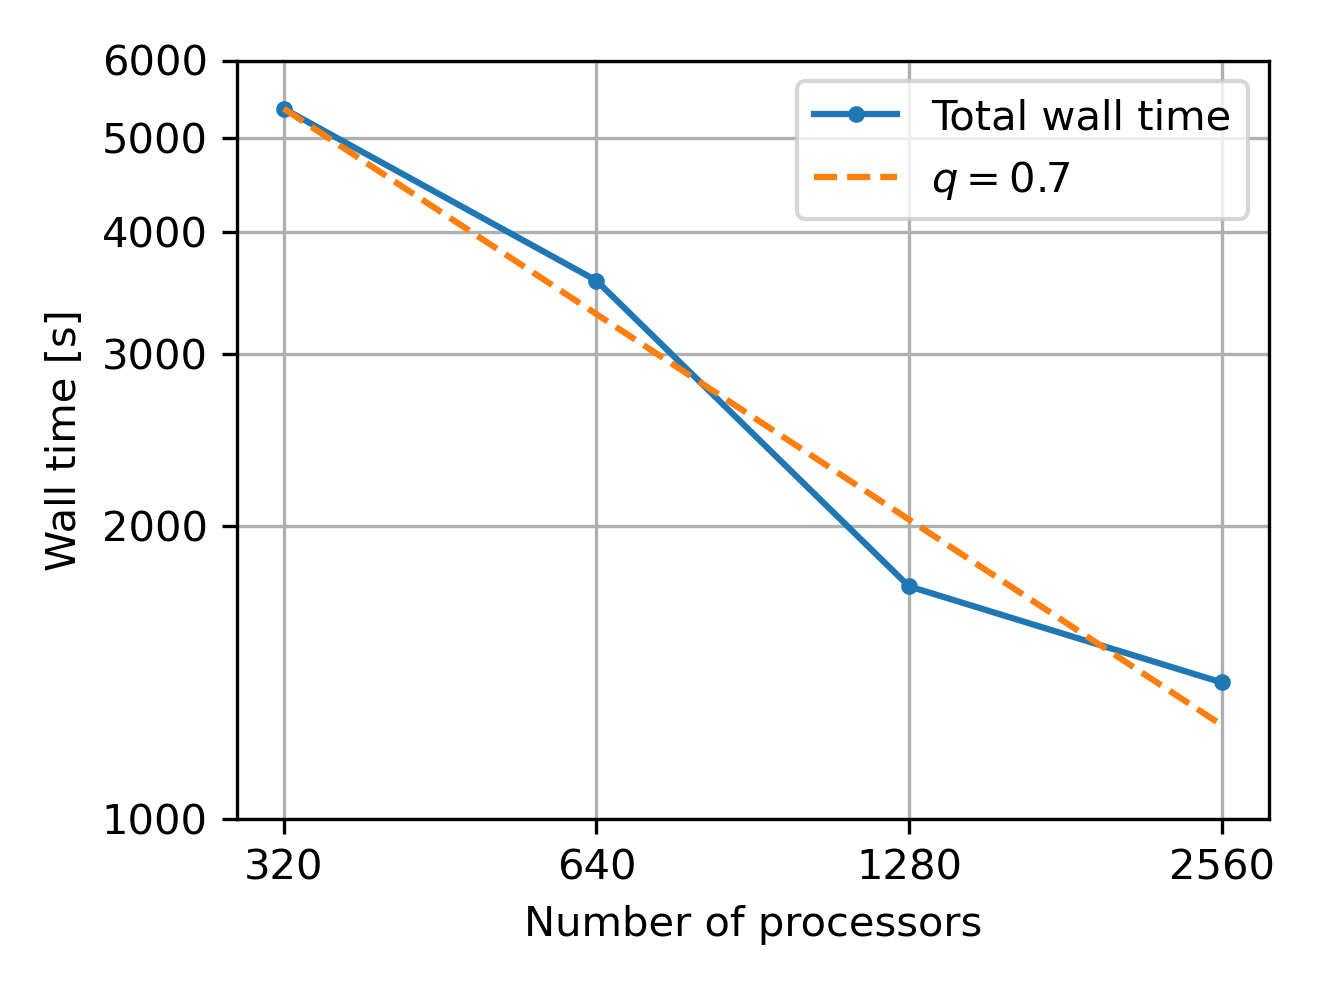
\includegraphics[width=\columnwidth]{scaling-total}
      \caption{Total wall time}
    \end{subfigure}
    \begin{subfigure}[b]{0.32\columnwidth}
      \centering
      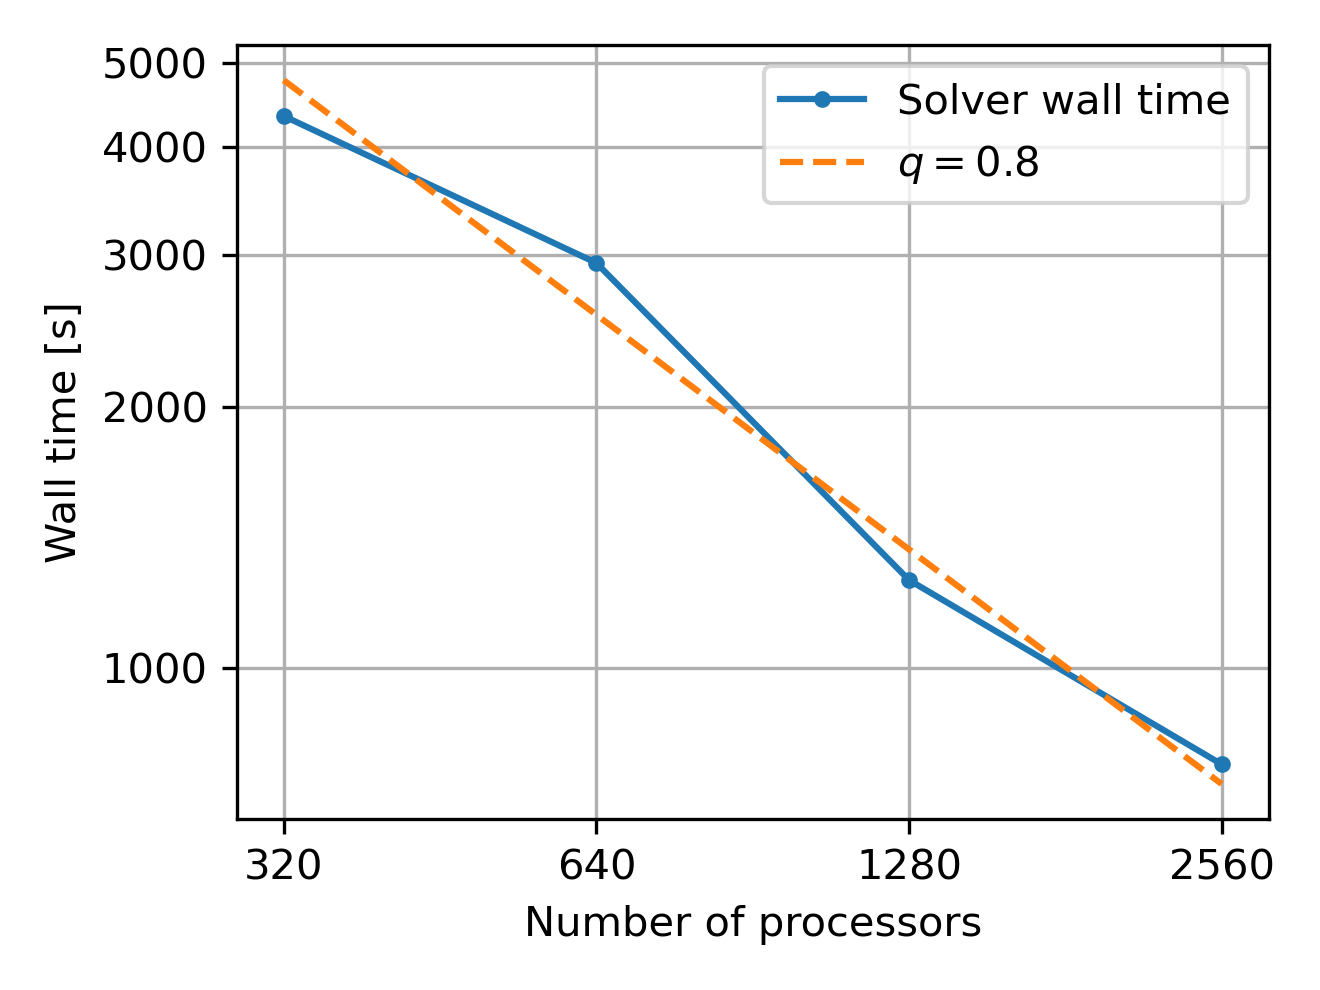
\includegraphics[width=\columnwidth]{scaling-solver}
      \caption{Solver wall time}
    \end{subfigure}
    \begin{subfigure}[b]{0.32\columnwidth}
      \centering
      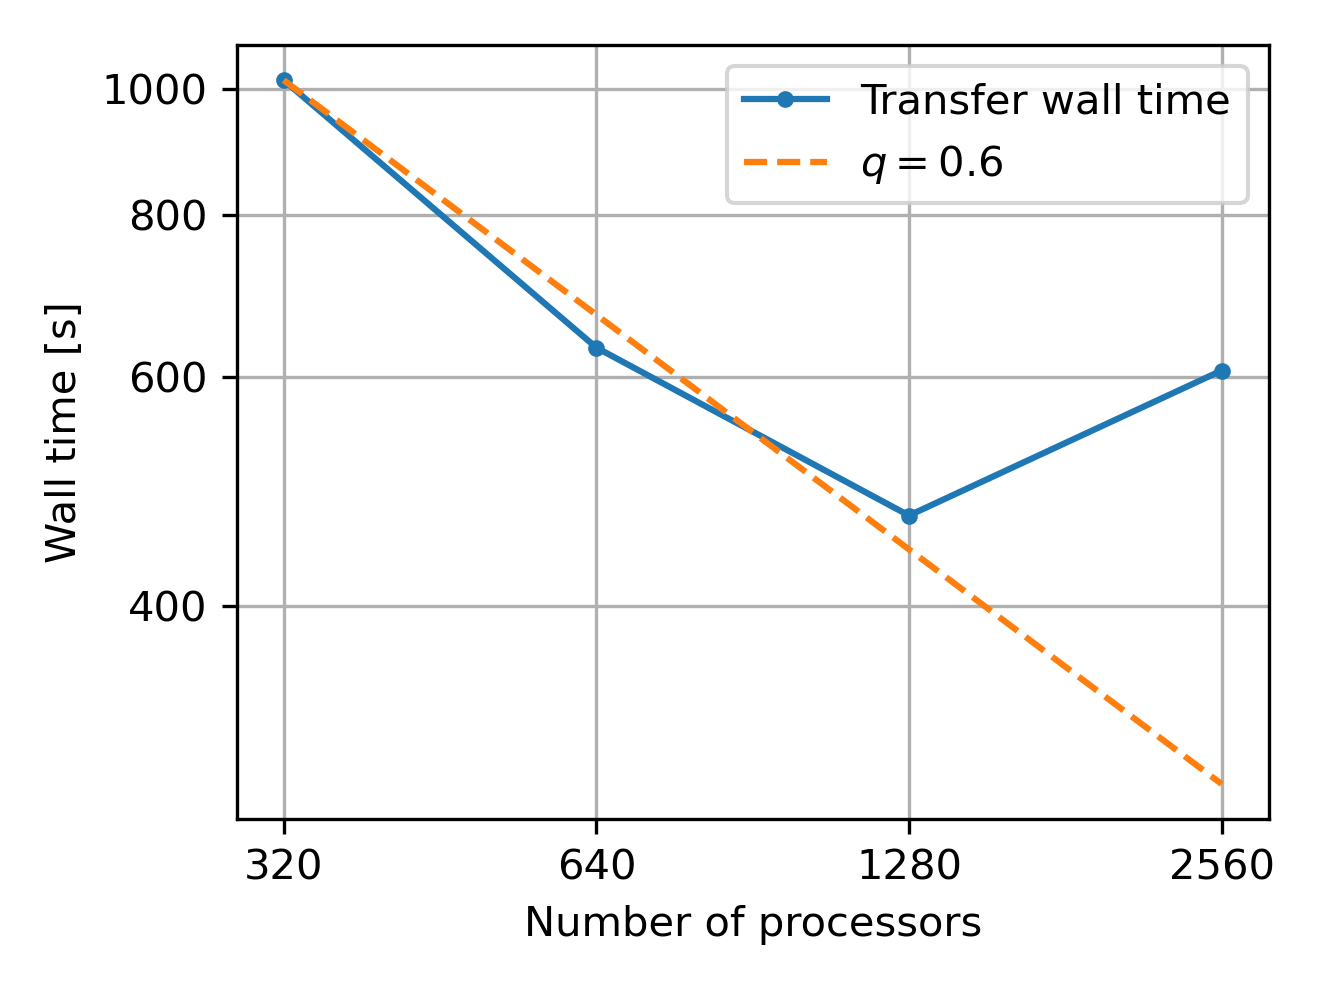
\includegraphics[width=\columnwidth]{scaling-transfer}
      \caption{Transfer wall time}
    \end{subfigure}
    \caption{The total, solver, and transfer wall time of hybrid method simulations of the 3-D
    quarter-core model on 10, 20, 40, and 80 compute nodes (32 processors per node) of the Polaris
    supercomputer. All axes are in log scale.}
    \label{fig:scaling}
  \end{figure}
\end{frame}
